\chapter{Design Problem: An Optical Receiver}

Photonics is a relatively new field, but the increasing possibility of incorporating photonics elements on chip with the electronics has led to optical circuits becoming a research hotspot. 

To demonstrate the capabilities of BAG, an optical receiver design from concept to verification is shown.

\section{Problem Statement and Architecture}
Photonic communication systems transmit and receive data using light, meaning that the receiver element must be a photo diode. A reverse biased photo diode receiver element can be modeled as a current source with some capacitance in parallel. This is the ``input'', analogous to an antenna in typical RF receivers. For this design, the following arbitrary specs are required:
\begin{itemize}
\item GF14nm technology
\item A data rate of 25Gbps
\item A photo diode capacitance of 50fF
\item $40\mu A$ peak to peak photo diode current
\item $V_{DD}=0.8V$
\item Must use BAG for generation and the majority of testing
\end{itemize}

There are no power constraints or architecture constraints with the condition that any chosen architecture will be implemented in BAG. We will assume the photonics are already implemented, and we will also not simulate for temperature, voltage or process variations. Each transistor will be of a unit size, and only the number of fingers will change. Noise in general should be low, but there is no strict value requirement. We will see in the ``Future Work'' of Chapter 5 how this could be extended, and an example of how one could generalize the design procedure automatically.

\subsection{Architecture Choice and Concerns}
The architecture is based off the receiver in \cite{settaluri_photonic_nodate} and is shown below:
\begin{figure}[h]
\centering
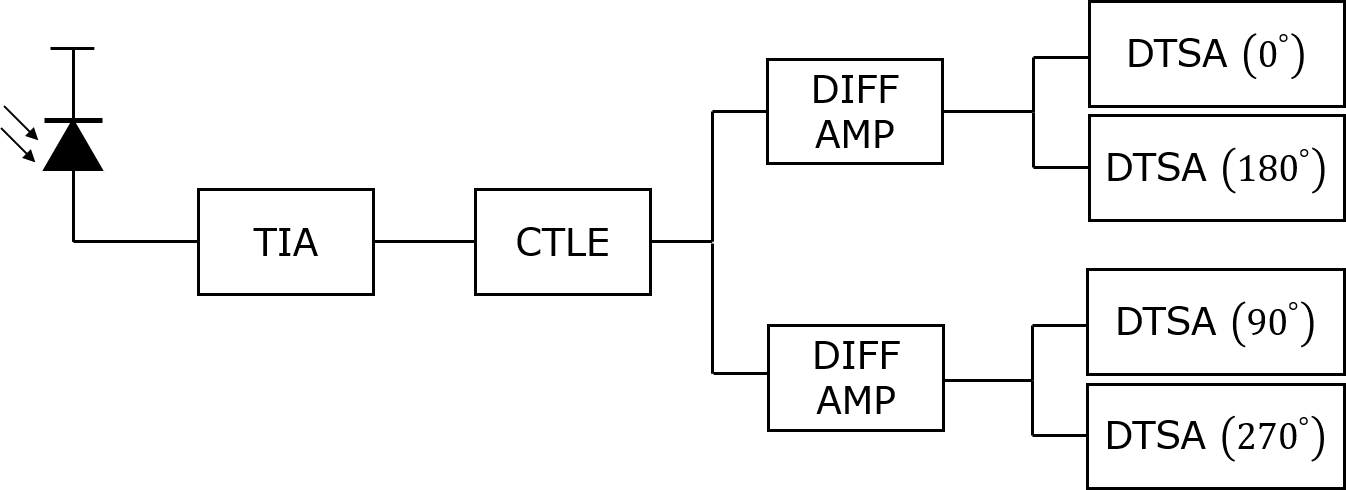
\includegraphics[width=0.7\textwidth]{architecture}
\caption{System architecture}
\label{fig:System Architecture}
\end{figure}

This receiver is a quad data rate (QDR) receiver with each comparator operating in $90^\circ$ phase offsets at a quarter of the clock rate to reduce the comparator constraints. Technically, only a single comparator clocked at 25GHz is necessary, however the time required for a comparator to decide between a 1 or 0 bit is finite, and mostly determined by device limitations rather than designer's choice. To meet the target, we use four comparators that operate only a quarter of the time to allow enough time for decision making and regeneration.This will be further discussed in following parts of this chapter.

Another design choice made is to drive the $0^\circ$ and $180^\circ$ offset comparators with the same preamp, and $90^\circ$and $270^\circ$ together. This was done to reduce the effect of back-injection of the clock into the circuit elements before it.

The transimpedance amplifier (TIA) is the main gain stage and is used to convert the incoming current waveform into a voltage. Since the TIA is the first block in the chain, the formula for cascaded noise figures

\begin{equation}
\label{friis}
F_{total}=F_1+\frac{F_2-1}{G_1}+\frac{F_3-1}{G_1G_2}+...
\end{equation}

(where $F_1$ and $G_i$ are the noise factor and gain of stage $i$ respectively) tells us we want the TIA to be high gain and low noise in order to reduce the overall noise factor of the system.

The TIA is followed by a continuous time linear equalizer (CTLE). A CTLE has a zero in its transfer function that can be placed at a specific frequency, which theoretically allows the designer to extend the bandwidth of previous stages as in figure \ref{fig:CTLE Operation}. One concern of the CTLE however, is that it can only, in general, shape the energy of the frequency spectrum. This means that usually to increase the gain at high frequency, we must throw away DC gain, as shown below:

\begin{figure}[h]
\centering
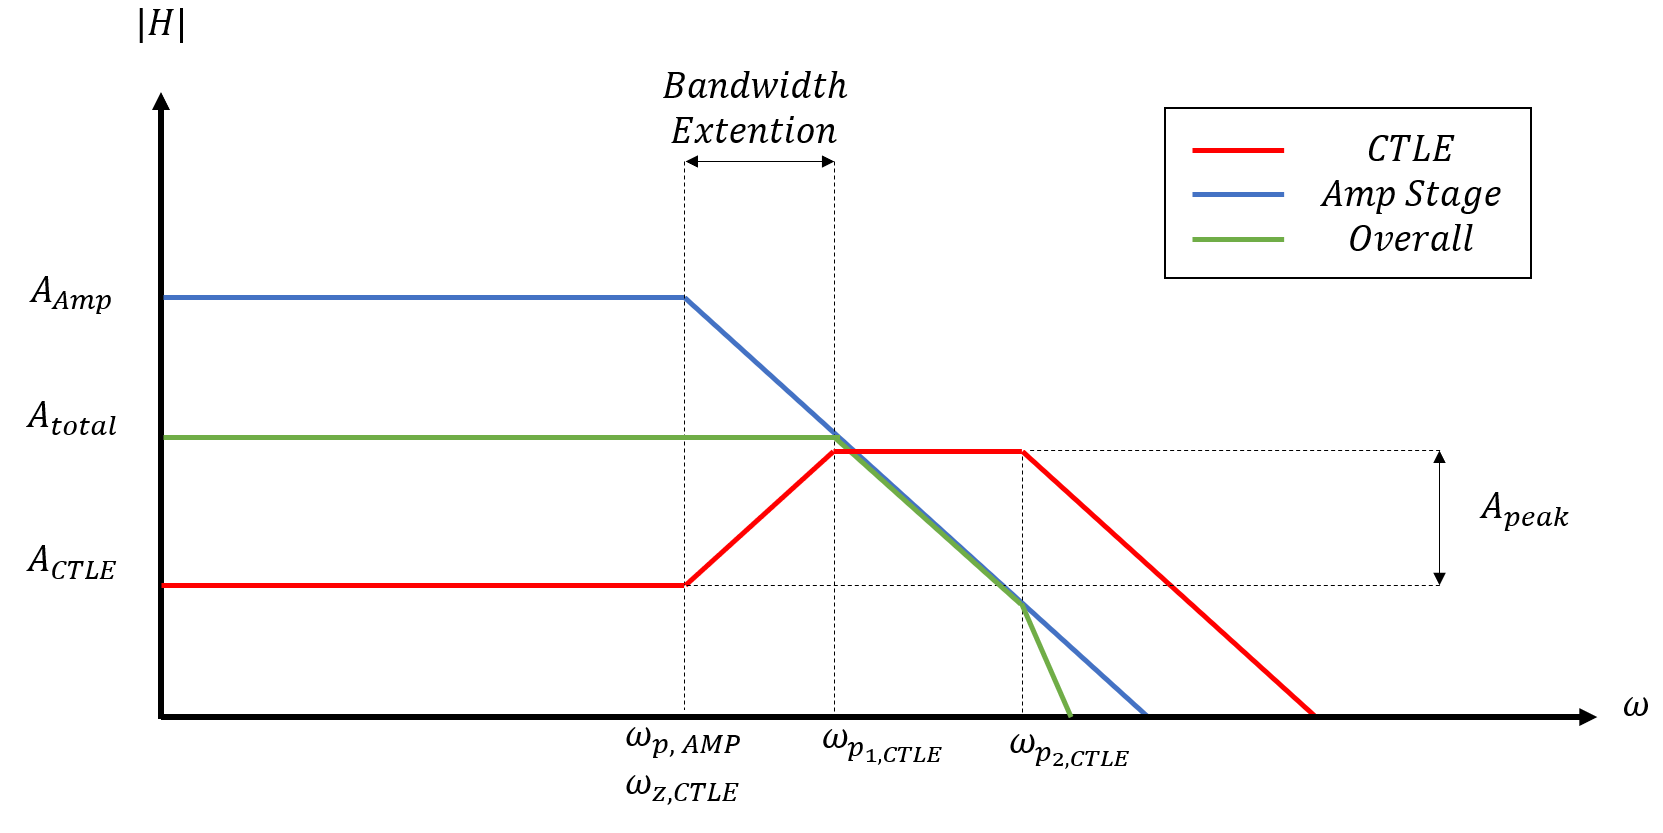
\includegraphics[width=0.8\textwidth]{ctle_operation}
\caption{CTLE effect on a generic one-pole system}
\label{fig:CTLE Operation}
\end{figure}

Since we are targeting 25Gbps, the empirical target bandwidth the front end receiver needs for a relatively optimal trade off in power and introduced ISI is $\approx 0.7\times$ the data rate, or roughly 17GHz \cite{settaluri_first_2017}. The bare minimum would be roughly half, or 12.5GHz. We will target somewhere in between. A good rule of thumb for comparators is that they need milivolts of signal swing to consistently measure correctly. The gain bandwidth product of the TIA is unlikely to be large enough to get a $40\mu A$ signal to roughly $10mV$ across a frequency range of 0Hz to 17GHz and be low noise, so we increase the TIA gain and lower the bandwidth so that even with the CTLE DC gain reduction, we can still get decent gain in conjunction with the CTLE bandwidth extension. 

The final stage before the comparators is a set of passively loaded differential amplifiers. Their purpose is threefold. The CTLE would have to simultaneously drive four comparators, which is a fairly large capacitive load. This limits the maximum achievable peaking gain by pushing in the second pole. Additionally, the comparators tend to inject their clock signal backwards which can impact the CTLE's operation periodically. The amplifiers serve as buffers which will isolate the kickback, and act as an intermediate step to reduce the amount of capacitance the CTLE has to drive. The DC gain is also expected to be too low due to the CTLE's reduction, so the amplifiers will provide a relatively small gain ($\approx 2\times$) to get as much swing as possible.


%\begin{figure}\centering
%\parbox{.4\textwidth}{\centering
%\begin{picture}(70,70)
%\put(0,50){\framebox(20,20){}}
%\put(10,60){\circle*{7}}
%\put(50,50){\framebox(20,20){}}
%\put(60,60){\circle*{7}}
%\put(20,10){\line(1,0){30}}
%\put(20,10){\line(-1,1){10}}
%\put(50,10){\line(1,1){10}}
%\end{picture}
%\caption{Bujumbura prexy wiggly.}}
%\hfill
%\parbox{.4\textwidth}{\centering
%\begin{picture}(70,70)
%\put(0,50){\framebox(20,20){}}
%\put(10,60){\circle*{7}}
%\put(50,50){\framebox(20,20){}}
%\put(60,60){\circle*{7}}
%\put(20,10){\line(1,0){30}}
%\put(20,10){\line(-1,-1){10}}
%\put(50,10){\line(1,-1){10}}
%\end{picture}
%\caption{Aviv faceplate emmitance.}}
%\end{figure}

\section{Transimpedance Amplifier}
The TIA is implemented as a pseudo-differential structure as two CMOS inverters with resistive feedback. 
\begin{figure}[h]
\centering
\ctikzset{tripoles/mos style/arrows}
\begin{circuitikz}[american voltages]
\draw (3, 2) node[american not port](n){};
\draw (3, 3.5) node[american not port](p){};
\draw (p.out) to[short] (4, 3.5) |- (4, 4.5) to[R, l_=$R_{fb}$] (2, 4.5);
\draw (p.in) -| (2, 4.5);
\draw (n.out) to[short] (4, 2) |- (4, 1) to[R, l=$R_{fb}$] (2, 1);
\draw (n.in) -| (2, 1);
\draw (p.out) to[short, -o] (5, 3.5) to[open, v^=$V_{out}$, -o] (5, 2) to[short] (n.out);
\draw (p.in) to[short] (-1, 3.5) to[american current source, l_=$I_{DC}$] (-1, 2) to[short] (-1, 1.5) node[ground]{};
\draw (-1, 3.5) to[short, *-] (-1, 4) to[pDo] (-1, 4.5) to[short] (-1, 5) node[rground, yscale=-1]{} to[open] (-1, 5.5) node[above]{$V_{DD}$};
\draw (-1, 4.75) to[short] (0, 4.75) to[C, l=$C_{pd}$] (0, 3.5);
\draw (n.in) to[short] (1, 2) to[american current source, l_=$I_{DC}$] (1, 0.5) to[short] (1, 0) node[ground]{};
\end{circuitikz}
\label{TIA Schematic}
\caption{TIA Schematic}
\end{figure}

The purpose of implementing the TIA is due to the usage in both \cite{mehta_12gb/s_2016} and \cite{settaluri_photonic_nodate}. The photodetector can split into a differential input that achieves good performance. At DC, if $I_{DC}=0$ then the input and output common mode voltages are equal. The purpose of the DC current source is to force the output common mode to be higher if desired. Since the output will sit about mid-rail, that may not be enough to bias the input of the CTLE, so we will need DC current through $R_{fb}$ to force this difference.

If we assume the inverters are an amplifier with gain $-A_v$ then the input impedance can be found by using Miller's theorem. 
\begin{equation}
\label{TIA input impedance}
Z_{in}=Z_{C_{pd}}||(1+A_v)R_{fb}
\end{equation}
which simplifies to 
\begin{equation}
\label{TIA input impedance}
\frac{(1+A_v)R_{fb}}{1+j\omega (1+A_v)C_{pd}R_{fb}}
\end{equation}
Thus the input pole should be roughly at
\begin{equation}
\label{TIA input pole}
\omega_p=\frac{1}{(1+A_v)R_{fb}C_{pd}}
\end{equation}

\begin{figure}[h]
\centering
\ctikzset{tripoles/mos style/arrows}
\begin{circuitikz}[american voltages]
\draw (0, 0) to[american current source, v=$v_{gs}$, l=$i_{in}$] (0, 2.5);
\draw (0, 0) node[ground]{};
\draw (0, 2.5) to[R, l=$R_{fb}$] (2, 2.5);
\draw (2, 2.5) to[american controlled current source, l=$g_{mn} v_{gs}$] (2, 0);
\draw (2, 2.5) to[short] (4.5, 2.5) to[american controlled current source, l=$g_{mp} v_{gs}$] (4.5, 0);
\draw (4.5, 2.5) to[short] (7, 2.5) to[R, l=$r_{on}||r_{op}$] (7, 0);
\draw (7, 2.5) to[short, -o] (8, 2.5) node[label={[font=\footnotesize]0:$v_{out}$}] {};
\draw (7, 0) to[short] (0, 0);
\end{circuitikz}
\caption{TIA Small Signal Model}
\label{fig:PLEASE}
\end{figure}
From the small signal model of one half of the circuit (shown in figure \ref{fig:PLEASE}, ignoring $C_{pd}$) we can derive the gain. KCL at the output node gives
\begin{equation}
\label{TIA gain KCL}
\frac{v_{out}}{r_{on}||r_{op}}+(g_{mn}+g_{mp})(i_{in}R_{fb}+v_{out})-i_{in}=0
\end{equation}
which simplifies to
\begin{equation}
\label{TIA gain full}
\frac{v_{out}}{i_{in}}=\frac{R_{fb}(g_{mn}+g_{mp})-1}{-(g_{mn}+g_{mp})-\frac{1}{r_{on}||r_{op}}}
\end{equation}
If we assume $R_{fb}$ and $r_{on}||r_{op}$ are both much larger than 1, then the transfer function simplifies to
\begin{equation}
\label{TIA gain}
|\frac{v_{out}}{i_{in}}|=R_{fb}
\end{equation}
The gain is then approximately just $R_{fb}$. For a given choice of $R_{fb}$, we then use BAGs rapid iteration to sweep for transistor widths. As the size increases, device parasitics become dominant over the external capacitances, so there is an optimal size for bandwidth. Once the maximum bandwidth is found, this sets the device sizes. Since we know the CTLE can only get a couple of GHz of bandwidth extension, we can calculate and then sweep the TIA resistor to see what resistance gives a bandwidth of around 9GHz. If we assume the CTLE will cut the DC gain by roughly a third, and we can get about 1.5x amplification from the preamps, then the overall gain should still be high enough for the comparator.

To set the output common mode, we can assume the input will be around mid-rail, so the output can be approximated as follows:
\begin{equation}
\label{tia_dc}
\frac{V_{o}-\frac{V_{DD}}{2}}{R_{fb}}=I_{DC}
\end{equation}
In order to bias the CTLE input, we want this to potentially be a little higher than midrail since the $V_{GS}$ needs to be large enough to give headroom to the tail transistors. Plugging into equation \ref{tia_dc} gives a starting point that can then be swept using BAG for better accuracy. Post-PEX hand-simulation is then used to fine tune the current the get the desired result. Note that by increasing the output common mode, the gain can reduce. This means that the resistance might need to be higher than anticipated. This is also determined by simulating BAG generated instances.

We were able to achieve a gain of 1500 with a bandwidth of 8.55GHz. In order to shift the common mode, $I_{DC}$ was set to $55\mu A$.

\section{Continuous Time Linear Equalizer}
A CTLE is a simple amplifier, degenerated by a parallel resistor capacitor combination as shown below:
\begin{figure}[h]
\centering
\ctikzset{tripoles/mos style/arrows}
\begin{circuitikz}[american voltages]
\draw (1, 1) node[nmos](n_in){};
\draw (3, 1) node[nmos, xscale=-1](p_in){};
\draw (n_in.drain) to[R, l=$R_d$] (1, 3.5);
\draw (1, 3.5) to[short] (2, 3.5) node[above]{$V_{DD}$};
\draw (2, 3.5) to[short] (3, 3.5) to[R, l=$R_d$] (p_in.drain);
\draw (n_in.source) to[C, *-,  l=$C_s$] (p_in.source);
\draw (n_in.source) to[short] (1, -1) to[R, *-*, l=$R_s$] (3, -1) to[short, -*] (p_in.source);
\draw (1, -2) node[nmos](n_tail){};
\draw (n_tail.drain) to[short] (1, -1);
\draw (3, -2) node[nmos](p_tail){};
\draw (p_tail.drain) to[short] (3, -1);
\draw (n_tail.source) to[short] (1, -3) to[short, -*] (2, -3) node[ground]{};
\draw (2, -3) to[short] (3, -3) to[short] (p_tail.source);
\draw (-1, -2) node[nmos, xscale=-1](bias){};
\draw (bias.source) to[short] (-1, -3) to[short] (2, -3);
\draw (bias.drain) to[short, -o] (-1, 0) node[above]{$I_{bias}$};
\draw (-1, -1) to[short, *-] (0, -1) to[short, -*] (bias.gate);
\draw (bias.gate) to[short] (p_tail.gate);
\draw (n_in.gate) node[label={[font=\footnotesize]180:$V_{in}$}] {};
\draw (p_in.gate) node[label={[font=\footnotesize]0:$V_{ip}$}] {};
\draw (p_in.drain) to[short, -o] (2.5, 1.77) to[open, v=$V_{out}$] (1.5, 1.77) to[short, o-] (n_in.drain);
\end{circuitikz}
\label{CTLE Schematic}
\caption{CTLE Schematic}
\end{figure}

Since we know the pole location of the TIA after simulation, we can design the CTLE to have its zero in close proximity. Firstly, we draw the approximate differential mode half circuit:

\begin{figure}[h]
\centering
\ctikzset{tripoles/mos style/arrows}
\begin{circuitikz}[american voltages]
\draw (1, 1) node[nmos](n_in){};
\draw (n_in.drain) to[R, l=$R_d$] (1, 3.5);
\draw (1, 3.5) node[rground, yscale=-1]{} to[open] (1, 4) node[above]{$V_{DD}$};
\draw (n_in.source) to[short] (1, 0) to[short] (0.5, 0) to[R, l_=$\frac{R_s}{2}$] (0.5, -1.5);
\draw (n_in.source) to[short] (1, 0) to[short] (1.5, 0) to[C, l=$2C_s$] (1.5, -1.5);
\draw (1.5, -1.5) to[short, -*] (1, -1.5) to[short] (0.5, -1.5);
\draw (1, -1.5) node[ground]{};
\draw (n_in.drain) to[short, -o] (1.5, 1.77)  node[label={[font=\footnotesize]0:$V_{out}$}] {};
\draw (n_in.gate) node[label={[font=\footnotesize]180:$V_{in}$}] {};
\end{circuitikz}
\label{CTLE Half-Circuit}
\caption{CTLE Half-Circuit}
\end{figure}

which by inspection, we know
\begin{equation}
\label{Gm}
G_m=\frac{g_m}{1+g_m(\frac{R_s}{2}||\frac{Z_{C_s}}{2})}
\end{equation}
\begin{equation}
G_m=\frac{2g_m(1+j\omega R_sC_s)}{2+g_mR_s+2j\omega R_sC_s}
\end{equation}
We can also determine the output impedance by inspection
\begin{equation}
\label{Ro}
R_o\approx R_l||\frac{Z_{C_l}}{2}=\frac{R_d}{1+2j\omega R_d C_l}
\end{equation}
So the overall gain is then
\begin{equation}
\label{ctle_gain}
G_mR_o=\frac{2g_m(1+j\omega R_sC_s)R_d}{(2+g_m R_s+2j\omega R_sC_s)(1+2j\omega R_dC_l)}
\end{equation}
which puts the zero at 
\begin{equation}
\label{zero}
\omega_z=\frac{1}{R_sC_s}
\end{equation}
and the first pole at 
\begin{equation}
\label{pole_1}
\omega_{p1}=\frac{1+gm\frac{R_s}{2}}{R_sC_s}
\end{equation}
with the second pole at
\begin{equation}
\label{pole_2}
\omega_{p2}=\frac{1}{2R_dC_l}
\end{equation}
and lastly, the ideal peaking gain should be 
\begin{equation}
\label{peak gain}
A_{peak}=g_mR_d
\end{equation}
From these equations, we can choose the values of the degeneration components and pullup resistors to place the zero and set the peak gain. We want the second pole to be far away at roughly 20GHz or more, which fixes $R_d$ for a given $C_l$. If we want a peak gain of around 2, that then fixes the required $g_m$, which for an assumed $V_{ov}$ of 200mV, fixes the bias current and transistor sizes. We will (quite conservatively) assume the input to each amplifier is 10fF, so the total load is 20fF. Through BAG, we can sweep component values near the desired points to get more accurate results.

Using the above steps, we were able to achieve a bandwidth extension of about 4GHz with a DC gain of roughly 0.6. When placed in succession to the TIA, the overall gain reduces to about 850 with a bandwidth extension to about 13.5GHz.

\section{Preamplifiers}
The preamplifiers are implemented as passively-loaded differential amplifiers as shown below. The main purpose is to serve as a buffer between the CTLE and the DTSAs. The DTSAs will provide a fairly substantial capacitive load to the CTLE as well as back-inject their clock, which is undesired. The preamplifiers ideally will have a gain of around 2, but we will target a gain greater than 1. 

\begin{figure}[h]
\centering
\ctikzset{tripoles/mos style/arrows}
\begin{circuitikz}[american voltages]
\draw (1, 1) node[nmos](n_in){};
\draw (3, 1) node[nmos, xscale=-1](p_in){};
\draw (n_in.drain) to[R, l=$R_d$] (1, 3.5);
\draw (1, 3.5) to[short] (2, 3.5) node[above]{$V_{DD}$};
\draw (2, 3.5) to[short] (3, 3.5) to[R, l=$R_d$] (p_in.drain);
\draw (n_in.source) to[short] (1, 0) to[short, *-*] (3, 0) to[short] (p_in.source);
\draw (1, -1) node[nmos](n_tail){};
\draw (n_tail.drain) to[short] (1, 0);
\draw (3, -1) node[nmos](p_tail){};
\draw (p_tail.drain) to[short] (3, 0);
\draw (n_tail.source) to[short] (1, -2) to[short, -*] (2, -2) node[ground]{};
\draw (2, -2) to[short] (3, -2) to[short] (p_tail.source);
\draw (-1, -1) node[nmos, xscale=-1](bias){};
\draw (bias.source) to[short] (-1, -2) to[short] (2, -2);
\draw (bias.drain) to[short, -o] (-1, 0.5) node[left]{$I_{bias}$};
\draw (-1, 0) to[short, *-] (0, 0) to[short, -*] (bias.gate);
\draw (bias.gate) to[short] (p_tail.gate);
\draw (n_in.gate) node[label={[font=\footnotesize]180:$V_{in}$}] {};
\draw (p_in.gate) node[label={[font=\footnotesize]0:$V_{ip}$}] {};
\draw (p_in.drain) to[short, -o] (2.5, 1.77) to[open, v=$V_{out}$] (1.5, 1.77) to[short, o-] (n_in.drain);
\end{circuitikz}
\label{fig:preamp_schematic}
\caption{Preamp Schematic}
\end{figure}

Assuming the $r_o$ of the transistors are fairly large, then the gain of this amplifier is known to be
\begin{equation}
\label{preamp gain}
A_v=g_mR_d
\end{equation}
with the unity gain frequency at
\begin{equation}
\label{preamp ugb}
\omega_u=\frac{g_m}{C_l}
\end{equation}
Once we know the bandwidth of the CTLE, we can determine the required unity gain bandwidth for an overall gain of 2 at this frequency. Again assuming each DTSA provides 10fF of load, then we know $C_l$. This fixes the required $g_m$ and therefore the device sizes and bias current.

Following these steps, the amplifiers were able to obtain a gain of 1.5 up to 13.5GHz. This sets the entire front end chain to have an overall bandwidth of 13.5GHz and a gain of 1200. Assuming a $40\mu A$ peak-to-peak input current swing, this should be plenty for the comparator.

\section{Comparator}

The comparator is implemented as a double tail sense amplifier. 
\begin{figure}[h]
\centering
\ctikzset{tripoles/mos style/arrows}
\begin{circuitikz}[american voltages]
\draw (0, 0) node[nmos](tail_left){};
\draw (2, 0) node[nmos, xscale=-1](tail_right){};
\draw (tail_left.gate) node[label={[font=\footnotesize]180:$CLK$}] {};
\draw (tail_right.gate) node[label={[font=\footnotesize]0:$CLK$}] {};
\draw (tail_left.source) to[short] (0, -1) to[short, -*] (1, -1) node[ground]{} to[short] (2,-1) to[short] (tail_right.source);
\draw (0, 2) node[nmos](in_left){};
\draw (2, 2) node[nmos, xscale=-1](in_right){};
\draw (in_left.gate) node[label={[font=\footnotesize]180:$V_{in}$}] {};
\draw (in_right.gate) node[label={[font=\footnotesize]0:$V_{ip}$}] {};
\draw (in_left.source) to[short, -*] (tail_left.drain) to[short] (tail_right.drain) to[short, *-] (in_right.source);
\draw (0, 4) node[pmos, xscale=-1](left_reset){};
\draw (2, 4) node[pmos](right_reset){};
\draw (right_reset.gate) node[label={[font=\footnotesize]90:$CLK$}] {};
\draw (left_reset.gate) to[short] (right_reset.gate);
\draw (left_reset.drain) to[short, l=$D_{ip}$, -*] (in_left.drain);
\draw (right_reset.drain) to[short, l_=$D_{in}$, -*] (in_right.drain);
\draw (left_reset.source) to[short, l=$V_{DD}$] (right_reset.source);
\draw (-3, 8) node[nmos](left_switch){};
\draw (-1, 8) node[nmos, xscale=-1](inv_left_n){};
\draw (3, 8) node[nmos](inv_right_n){};
\draw (5, 8) node[nmos, xscale=-1](right_switch){}; 
\draw (-1, 10) node[pmos, xscale=-1](inv_left_p){};
\draw (-1, 12) node[pmos](p_switch_left){};
\draw (3, 10) node[pmos](inv_right_p){};
\draw (3, 12) node[pmos, xscale=-1](p_switch_right){};
\draw (in_left.drain) to[short] (-4, 2.77) to[short] (left_switch.gate);
\draw (in_right.drain) to[short] (6, 2.77) to[short] (right_switch.gate);
\draw (left_switch.source) to[short, -*] (inv_left_n.source) to[short, -*] (1, 7.23) to[short, -*] (inv_right_n.source) to[short] (right_switch.source);
\draw (1, 7.23) node[ground]{};
\draw (left_switch.drain) to[short, l=$V_{on}$] (inv_left_n.drain);
\draw (right_switch.drain) to[short, l_=$V_{op}$] (inv_right_n.drain);
\draw (inv_left_n.drain) to[short] (inv_left_p.drain);
\draw (inv_right_n.drain) to[short] (inv_right_p.drain);
\draw (inv_left_p.gate) to[short] (inv_left_n.gate);
\draw (inv_right_p.gate) to[short] (inv_right_n.gate);
\draw (inv_left_n.drain) to[short, *-*] (2.025, 8.77);
\draw (inv_right_p.drain) to[short, *-*] (-0.025, 9.225);
\draw (inv_left_p.source) to[short] (p_switch_left.drain);
\draw (inv_right_p.source) to[short] (p_switch_right.drain);
\draw (p_switch_left.source) to[short, l=$V_{DD}$] (p_switch_right.source);
\draw (p_switch_left.drain) to[short, *-*] (p_switch_right.drain);
\draw (p_switch_left.gate) node[label={[font=\footnotesize]180:$\overline{CLK}$}] {};
\draw (p_switch_right.gate) node[label={[font=\footnotesize]0:$\overline{CLK}$}] {};
\end{circuitikz}
\label{Double Tail Schematic}
\caption{Double Tail Schematic}
\end{figure}
\clearpage
The DTSA consists of a clocked differential pair that feeds into cross-coupled inverters. Much like the classic StrongArm sense-amp \cite{razavi_strongarm_2015}, the DTSA first precharges the $D_{in}$ and $D_{ip}$ nodes up to $V_{DD}$. After $CLK$ goes high, the input pairs activate and begin to drain charge from the parasitic capacitance at nodes $D_{in}$ and $D_{ip}$. Depending on which input is larger, one side will discharge faster which will turn off one of the switches connected to those nodes faster than the other. This sets the value in the cross-coupled inverters which is then reinforced through positive feedback. 

When $CLK$ goes low, the circuit resets and precharges the $D_{ip}/D_{in}$ nodes for the next cycle.

A typical cycle of the DTSA with a differential input of 10mV is plotted in figure \ref{fig:dtsa_op}. The clock is generated by taking ideal clocks and passing them through a chain of inverters to generate both the real $CLK$ and $\overline{CLK}$ signals.
\begin{figure}[h]
\centering
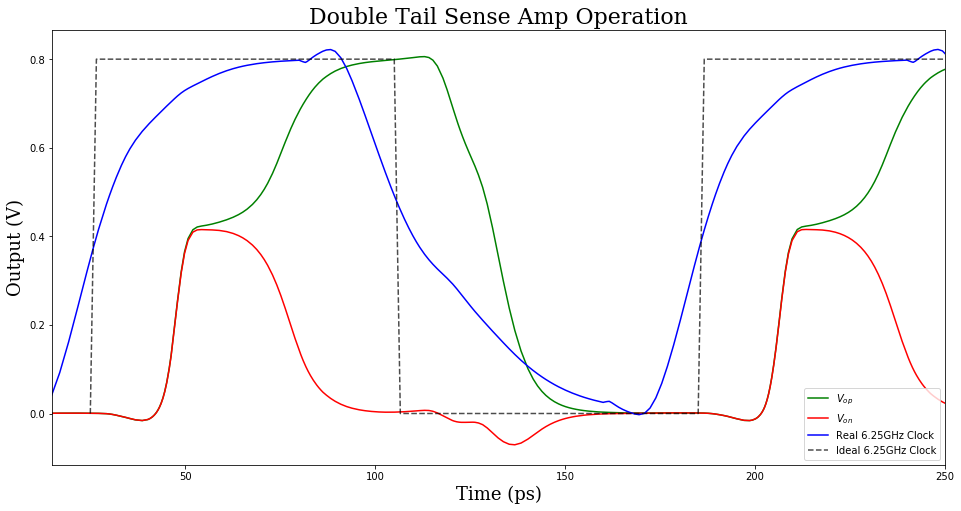
\includegraphics[width=\textwidth]{dtsa_one_cycle}
\caption{DTSA Typical Operation}
\label{fig:dtsa_op}
\end{figure}

The comparator usually is the first thing one would design, as its limitations generally set the required gain and noise specs for the front end. In this project, the comparator was designed last, since there is no power constraint. The rate at which voltage is reduced from $D_{ip}/D_{in}$ is based on the current through the input pairs. By increasing the size of the input pairs, we can create a voltage difference much more quickly (assuming there is no process offset in the input pairs) which allows even small inputs to be sensed before the cycle ends. Thus, as long as our input is on the order of milivolts, we should be able to sense this.

As a test, we determine what the approximate noise tolerance of the DTSA is. We input a small differential signal (about 1mV) and run a transient simulation with noise over many cycles. The fraction of incorrect evaluations to the total allows us to approximate $\sigma_n$, or the standard deviation of the noise tolerance for the DTSA. The results of this simulation are shown in figure \ref{fig:dtsa_noise}.
\begin{figure}[h]
\centering
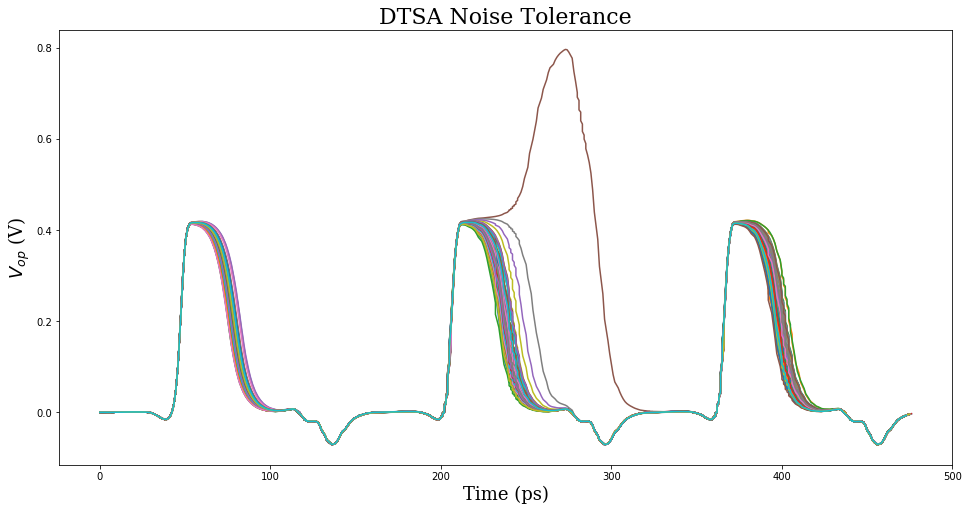
\includegraphics[width=\textwidth]{dtsa_noise_tolerance}
\caption{DTSA Noise}
\label{fig:dtsa_noise}
\end{figure}
With a differential input of 1mV, only one in 100 inputs failed. This implies two things. One, that 1mV is approximately $3\sigma_n$. This means we should budget about 3mV of the eye opening to noise tolerance for the DTSA for a BER of $10^{-12}$. Secondly, the DTSA minimum input voltage is less than 1mV, assuming no noise. Thus, as long as our input has a swing of 1mV in addition to the noise budget, then we should be able to obtain a bit error rate of $10^{-12}$. This, of course, ignores process variation. Process variation introduces an offset that affects the current in each branch. From a Monte Carlo simulation, one can find the average offset which can then additionally be added to the eye opening budget. There are also topologies that can correct for offset, which would not completely eliminate the issue, but would certainly reduce it.
\clearpage
\section{Design Verification}
There were four simulations done to verify the behavior of the entire receiver. Firstly, a simple AC simulation of the front-end chain up to the samplers in order to see if the circuit provides enough gain. This is shown in figure \ref{fig:afe_ac}
\begin{figure}[h]
\centering
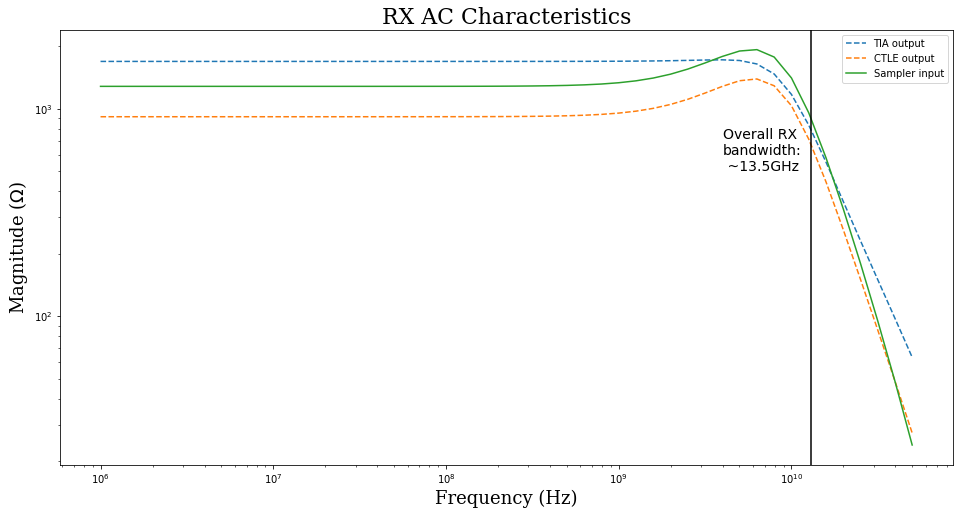
\includegraphics[width=\textwidth]{rx_ac_char}
\caption{AFE AC Performance}
\label{fig:afe_ac}
\end{figure}
\clearpage
To determine how much noise the amplifier chain introduces, an AC noise simulation was also run. The power spectral density is plotted in figure \ref{fig:psd}.
\begin{figure}[h]
\centering
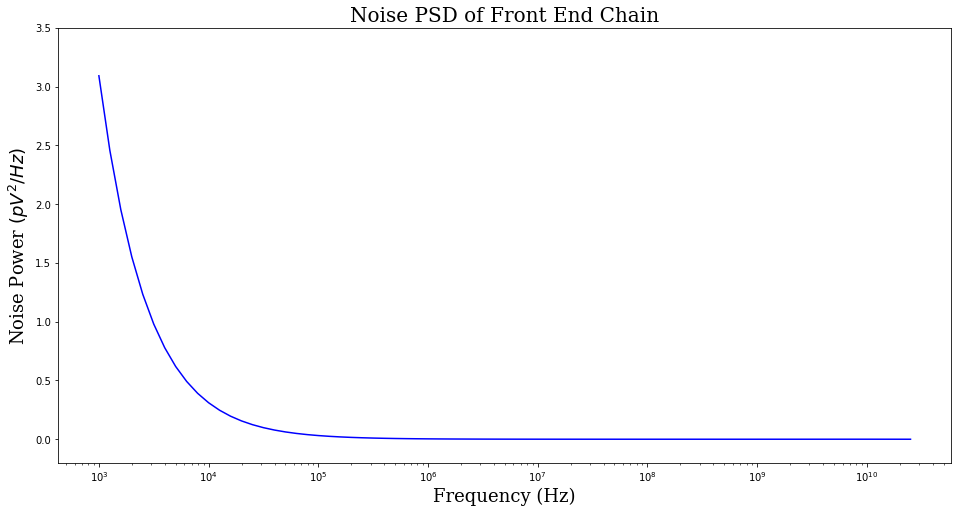
\includegraphics[width=\textwidth]{ac_noise}
\caption{Front End Noise PSD}
\label{fig:psd}
\end{figure}

Using Python to integrate this function up to 25GHz gives an rms noise of $4.6\mu V^2$, so the mean expected noise is then 2mV.
\clearpage
From the previous sections, we know that the minimum input is approximately 1mV with a noise tolerance of 3mV for a BER of $10^{-12}$. For an input of $40\mu A$ peak-to-peak, we achieve a gain of 1200 which puts the input amplitude at roughly 50mV peak-to-peak. This should be plenty. Unfortunately, the desired bandwidth was not met, although the bandwidth does surpass the theoretical minimum. This will mostly affect ISI performance, which will be seen in the next simulation.

To determine over many cycles how the AFE performs, we measure the eye diagram at the sampler inputs. This is shown in figure \ref{fig:eye}.
\begin{figure}[h]
\centering
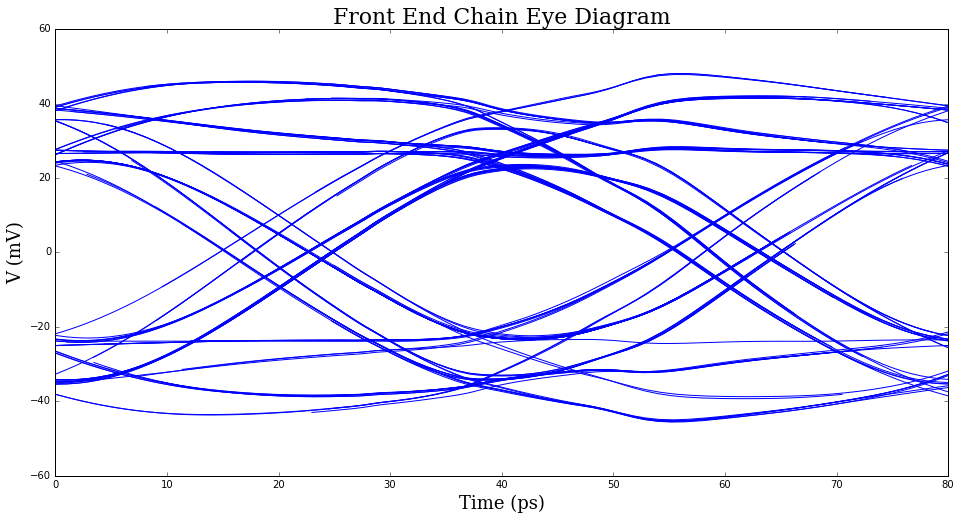
\includegraphics[width=\textwidth]{afe_eye}
\caption{Sampler Input Eye Diagram}
\label{fig:eye}
\end{figure}
As can be seen, there is a fairly large eye opening which surpasses the minimum required swing for proper evaluation.
\clearpage
Lastly, a PRBS32 pattern is fed into the receiver, and the sampler outputs are monitored in a transient simulation. Note that this architecture would not operate sufficiently due to the fact that the waveforms need to be adjusted in time to center the eye opening with the clock edges. This adjustment was done manually for this test. Also, since each sampler is only sampling once every 4 bits, the outputs are sliced and manually stitched together. A portion of the test input and output are shown in figure \ref{fig:prbs}. The patterns are clearly identical with only a time offset through the front end chain.
\begin{figure}[h]
\centering
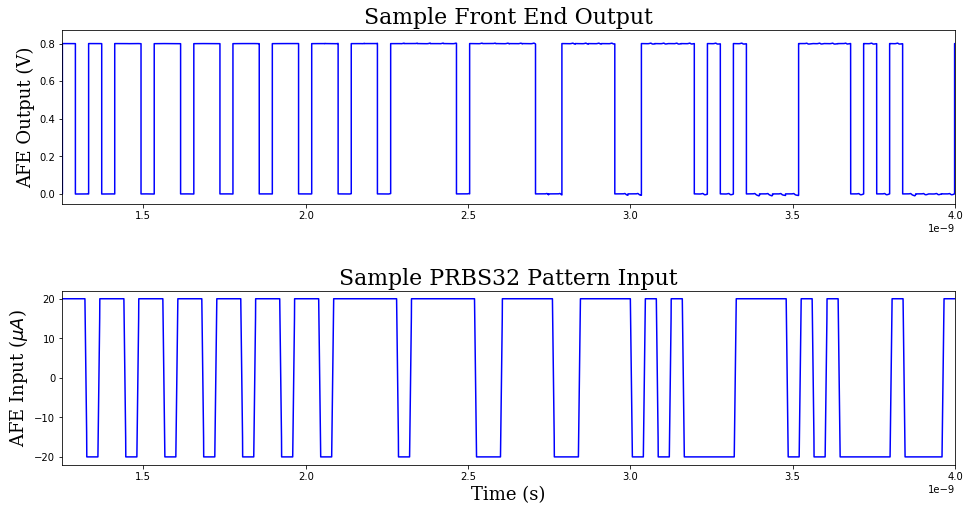
\includegraphics[width=\textwidth]{prbs_out}
\caption{PRBS Pattern Response}
\label{fig:prbs}
\end{figure}
\clearpage
